\section{Optimizing applications}

\begin{frame}
\frametitle{Measuring: strace}
\begin{itemize}
	\item Allows to trace all the system calls made by an
              application and its children.
	\item Useful to:
	\begin{itemize}
		\item Understand how time is spent in user space
		\item For example, easy to find file open attempts (\code{open()}),
		      file access (\code{read()}, \code{write()}), and
		      memory allocations (\code{mmap2()}). Can be done
		      without any access to source code!
		\item Find the biggest time consumers
		      (low hanging fruit)
		\item Find unnecessary work done in applications
		      and scripts. Example: opening the same file(s)
		      multiple times, or trying to open files that
		      do not exist.
	\end{itemize}
	\item Limitation: you can't trace the \code{init} process!
\end{itemize}
\end{frame}

\begin{frame}[fragile]
  \frametitle{strace}
  \begin{columns}
  \column{0.75\textwidth}
  \small
  System call tracer - \url{https://strace.io}
  \begin{itemize}
  \item Available on all GNU/Linux systems\\
        Can be built by your cross-compiling toolchain generator or by your build system.
  \item Allows to see what any of your processes is doing: accessing files, allocating memory...
        Often sufficient to find simple bugs.
  \item Usage:\\
    \code{strace <command>} (starting a new process)\\
    \code{strace -p <pid>} (tracing an existing process)\\
    \code{strace -c <command>} (statistics of system calls taking most time)
  \end{itemize}
  See \href{https://man7.org/linux/man-pages/man1/strace.1.html}{the strace manual} for details.
  \column{0.25\textwidth}
  \includegraphics[height=0.7\textheight]{common/strace-mascot.png}\\
  \tiny Image credits: \url{https://strace.io/}
  \end{columns}
\end{frame}

\begin{frame}[fragile]
  \frametitle{strace example output}
  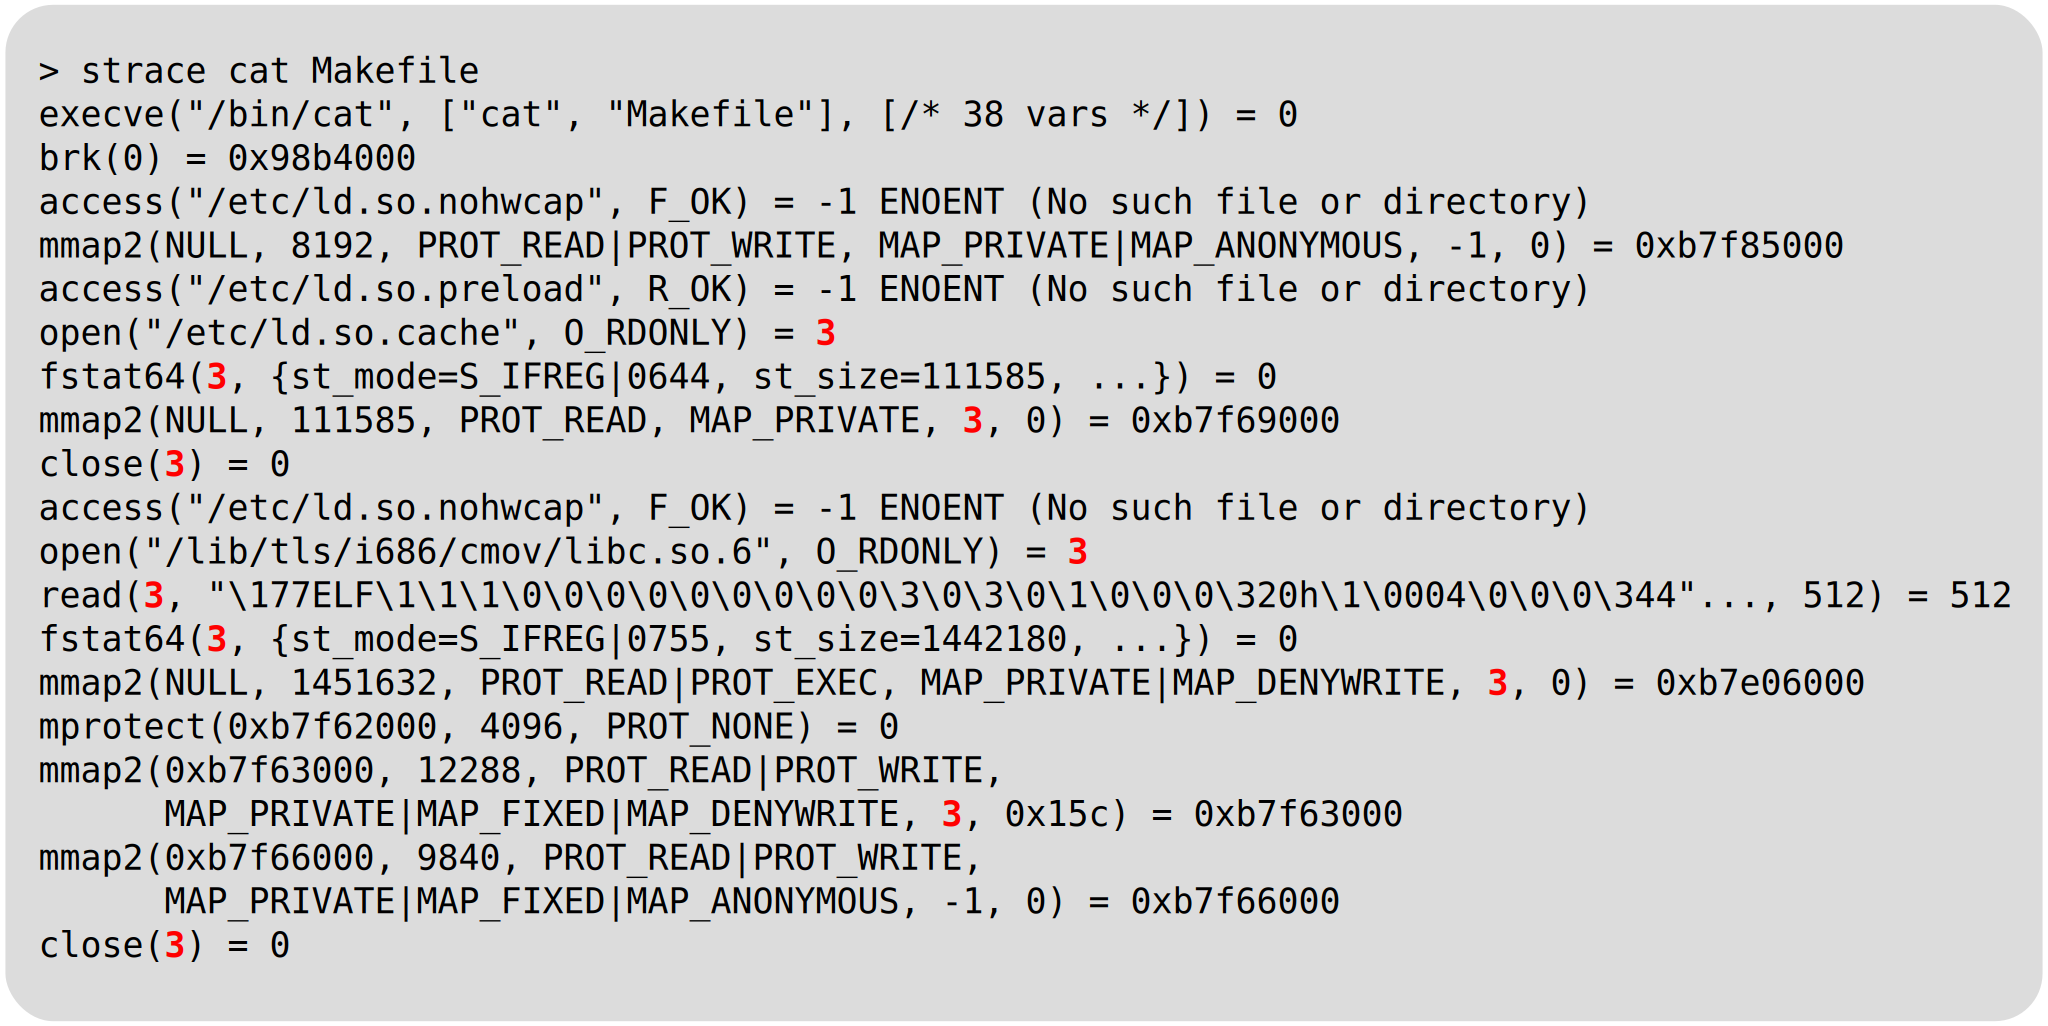
\includegraphics[height=0.75\textheight]{common/strace-output.pdf}\\
  Hint: follow the open file descriptors returned by \code{open()}.
  This tells you what files are handled by further system calls.
\end{frame}

\begin{frame}[fragile]
  \frametitle{strace -c example output}
  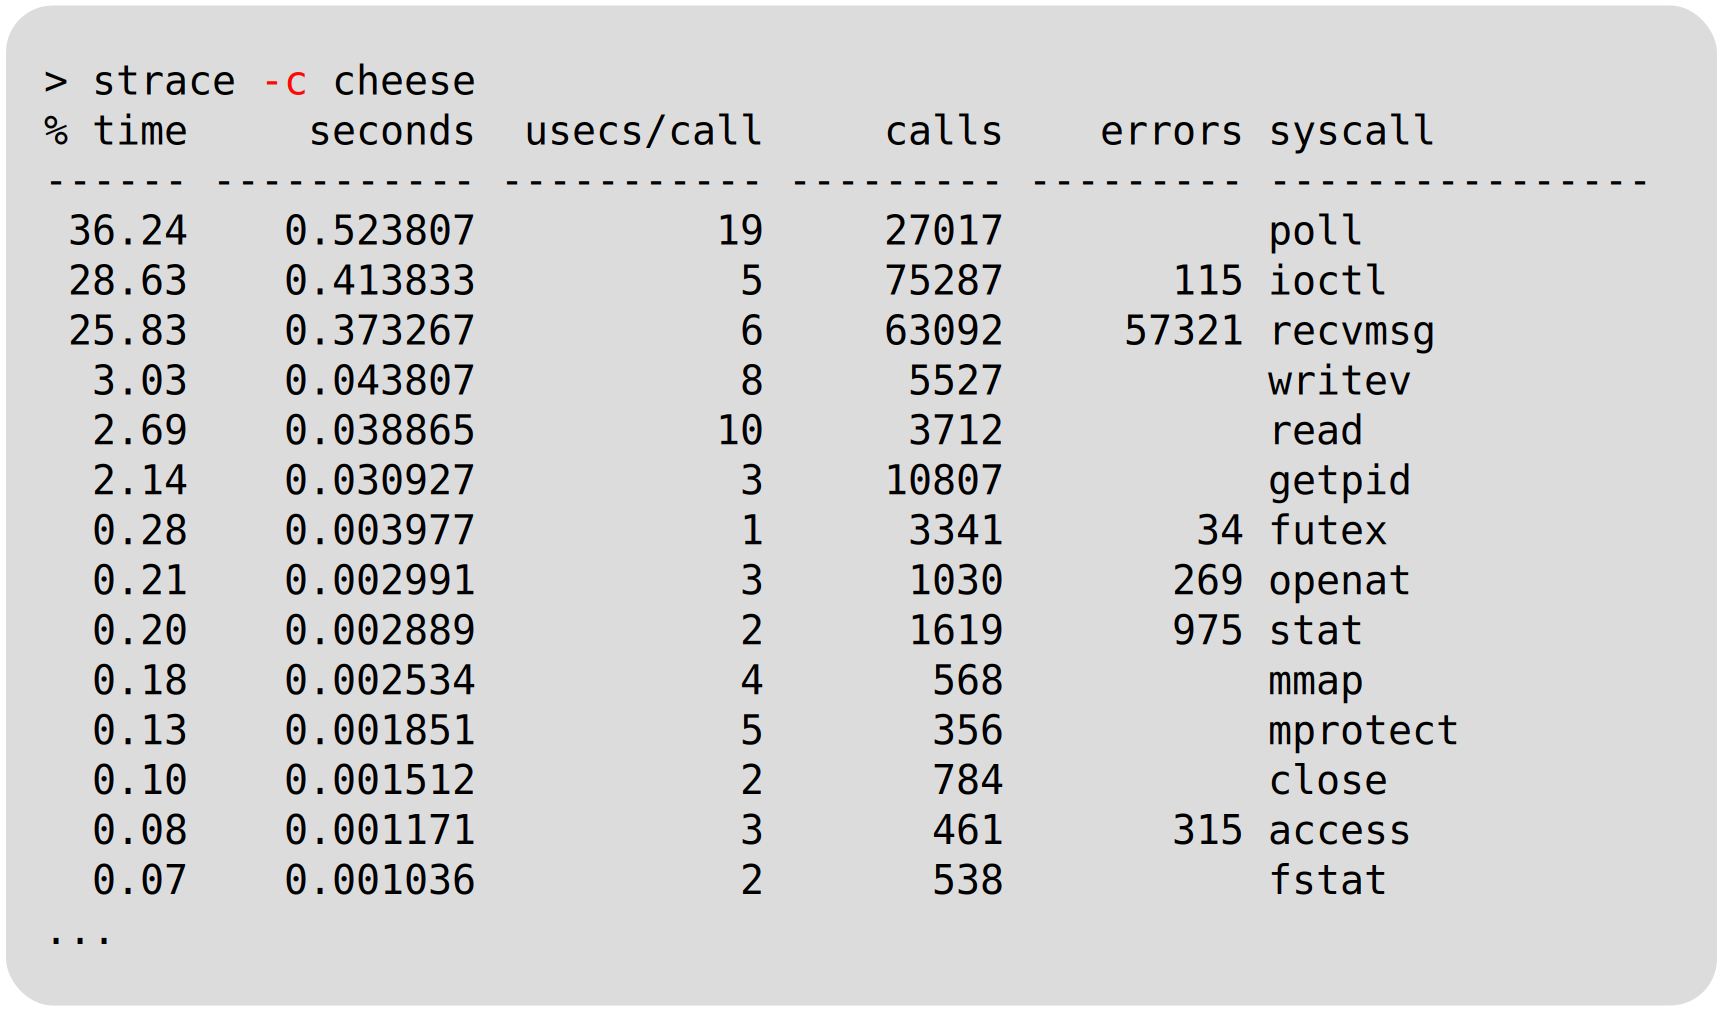
\includegraphics[height=0.8\textheight]{common/strace-c-output.pdf}
\end{frame}

\begin{frame}
  \frametitle{ltrace}
  A tool to trace library calls used by a program and all the signals
  it receives
  \begin{itemize}
  \item Very useful complement to \code{strace}, which shows only system
    calls. Library calls include system calls too!
  \item Of course, works even if you don't have the sources
  \item Allows to filter library calls with regular expressions, or
    just by a list of function names.
  \item Also offers a summary with its \code{-c} option.
  \item Manual page: \url{https://linux.die.net/man/1/ltrace}
  \item Works better with {\em glibc}. \code{ltrace} was broken
        with {\em uClibc} and may still be.
  \end{itemize}
  See \url{https://en.wikipedia.org/wiki/Ltrace} for details
\end{frame}

\begin{frame}[fragile]
  \frametitle{ltrace example output}
  \small
  \begin{block}{}
\begin{verbatim}
ltrace nedit index.html
sscanf(0x8274af1, 0x8132618, 0x8248640, 0xbfaadfe8, 0) = 1
sprintf("const 0", "const %d", 0) = 7
strcmp("startScan", "const 0") = 1
strcmp("ScanDistance", "const 0") = -1
strcmp("const 200", "const 0") = 1
strcmp("$list_dialog_button", "const 0") = -1
strcmp("$shell_cmd_status", "const 0") = -1
strcmp("$read_status", "const 0") = -1
strcmp("$search_end", "const 0") = -1
strcmp("$string_dialog_button", "const 0") = -1
strcmp("$rangeset_list", "const 0") = -1
strcmp("$calltip_ID", "const 0") = -1
\end{verbatim}
\end{block}
\end{frame}

\begin{frame}{Valgrind}
  \begin{columns}[T]
    \column{0.8\textwidth}
    \url{https://valgrind.org/}
    \begin{itemize}
    \item {\em instrumentation framework for building dynamic analysis tools}
      \begin{itemize}
      \item detect many memory management and threading bugs
      \item profile programs
      \end{itemize}
    \item Supported architectures: x86, x86-64, ARMv7, arm64, mips32,
      s390, ppc32 and ppc64
    \item Very popular tool especially for debugging memory issues
    \item Runs your program on a synthetic CPU $\rightarrow$
      significant performance impact (100 x slower on SAMA5D3!),
      but very detailed instrumentation
    \item Runs on the target. Easy to build with Yocto Project
	  or Buildroot.
    \end{itemize}
    \column{0.2\textwidth}
    
\includegraphics[width=\textwidth]{common/valgrind1.png}
  \end{columns}
\end{frame}

\begin{frame}{Valgrind tools}
  \begin{itemize}
  \item {\em Memcheck}: detects memory-management problems
  \item {\em Cachegrind}: cache profiler, detailed simulation of the
    I1, D1 and L2 caches in your CPU and so can accurately pinpoint
    the sources of cache misses in your code
  \item {\em Callgrind}: extension to Cachegrind, provides extra
    information about call graphs
  \item {\em Massif}: performs detailed heap profiling by taking
    regular snapshots of a program's heap
  \item {\em Helgrind}: thread debugger which finds data races in
    multithreaded programs. Looks for memory locations accessed by
    multiple threads without locking.
  \item More at \url{https://valgrind.org/info/tools.html}
  \end{itemize}
\end{frame}

\begin{frame}[fragile]{Valgrind examples}
  \begin{itemize}
  \item {\em Memcheck}
    \begin{block}{}
      {\tiny
\begin{verbatim}
$ valgrind --leak-check=yes <program>
  ==19182== Invalid write of size 4
  ==19182==    at 0x804838F: f (example.c:6)
  ==19182==    by 0x80483AB: main (example.c:11)
  ==19182==  Address 0x1BA45050 is 0 bytes after a block of size 40 alloc'd
  ==19182==    at 0x1B8FF5CD: malloc (vg_replace_malloc.c:130)
  ==19182==    by 0x8048385: f (example.c:5)
  ==19182==    by 0x80483AB: main (example.c:11)
\end{verbatim}
      }
    \end{block}

  \item {\em Callgrind}
    \begin{block}{}
      {\tiny
\begin{verbatim}
$ valgrind --tool=callgrind --dump-instr=yes --simulate-cache=yes --collect-jumps=yes <program>
$ ls callgrind.out.*
callgrind.out.1234
$ callgrind_annotate callgrind.out.1234
\end{verbatim}
      }
    \end{block}
  \end{itemize}
\end{frame}

\begin{frame}{Kcachegrind - Visualizing Valgrind profiling data}
  \begin{center}
    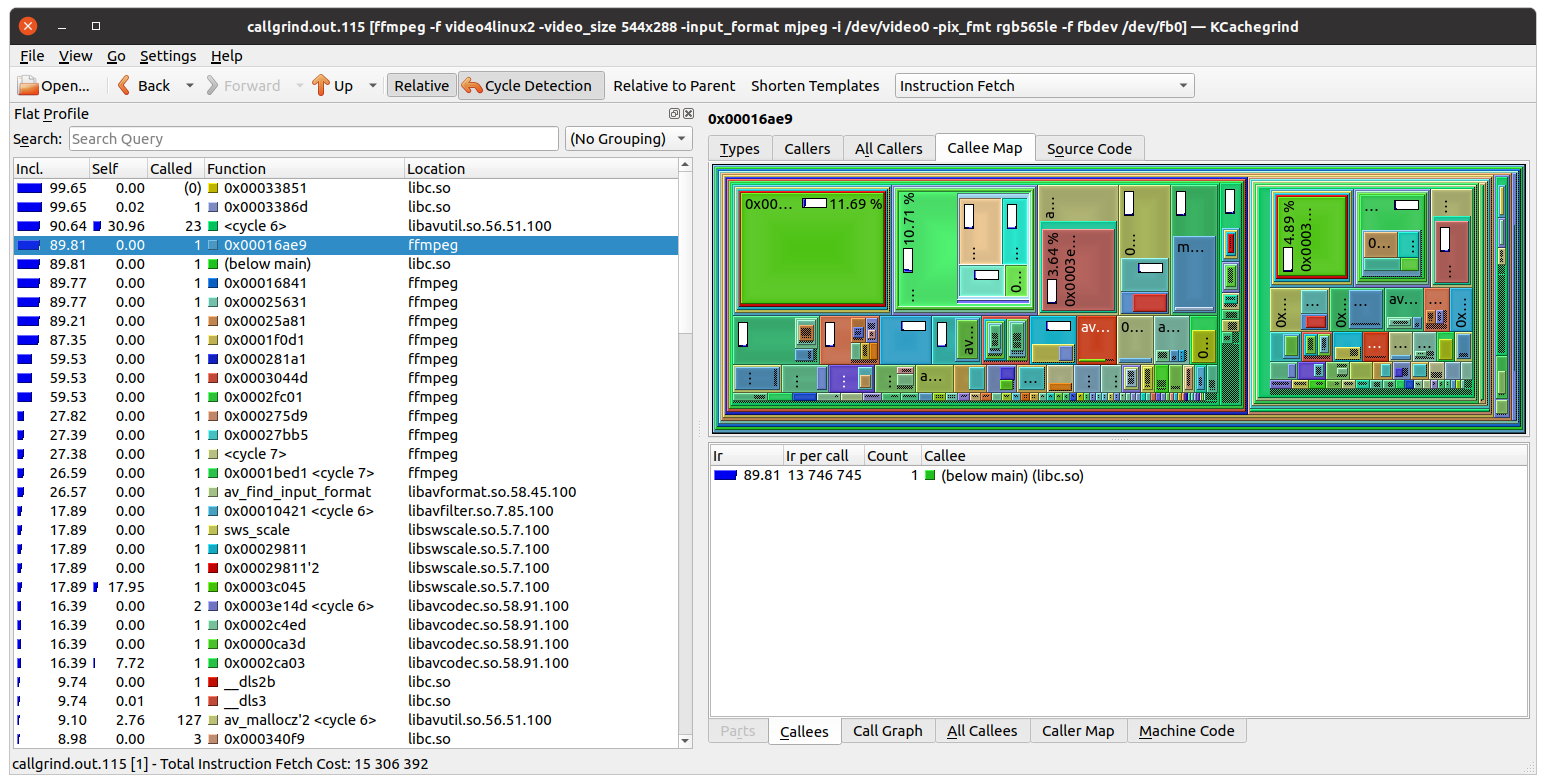
\includegraphics[height=0.8\textheight]{common/kcachegrind.png}
    \url{https://github.com/KDE/kcachegrind}
  \end{center}
\end{frame}


\begin{frame}[fragile]
\frametitle{perf}
\begin{itemize}
	\item Uses hardware performance counters
	\item \kconfig{CONFIG_PERF_EVENTS} and \kconfig{CONFIG_HW_PERF_EVENTS}
	\item User space tool: \code{perf}. It is part of the kernel
		sources so it is always in sync with your kernel.
	\item Usage:
	\begin{block}{}
\begin{verbatim}
perf record /my/command
\end{verbatim}
	\end{block}
	\item Get the results with:
	\begin{block}{}
\begin{verbatim}
perf report
\end{verbatim}
	\end{block}
\end{itemize}
\end{frame}

\begin{frame}[fragile]
\frametitle{perf report output}
\begin{block}{}
\tiny
\begin{verbatim}
# To display the perf.data header info, please use --header/--header-only options.
#
#
# Total Lost Samples: 0
#
# Samples: 5K of event 'cycles'
# Event count (approx.): 1392529663
#
# Overhead  Command  Shared Object             Symbol
# ........  .......  ........................  ....................................
#
    10.72%  ffmpeg   [kernel.kallsyms]         [k] video_get_user
    10.60%  ffmpeg   [kernel.kallsyms]         [k] vector_swi
     4.76%  ffmpeg   libc-2.31.so              [.] ioctl
     4.22%  ffmpeg   [kernel.kallsyms]         [k] __se_sys_ioctl
     3.81%  ffmpeg   [kernel.kallsyms]         [k] __video_do_ioctl
     3.42%  ffmpeg   libavformat.so.58.45.100  [.] avformat_find_stream_info
     2.83%  ffmpeg   [kernel.kallsyms]         [k] video_usercopy
     2.70%  ffmpeg   libc-2.31.so              [.] cfree
     2.58%  ffmpeg   [kernel.kallsyms]         [k] __fget_light
     2.53%  ffmpeg   libpthread-2.31.so        [.] __errno_location
     2.40%  ffmpeg   [kernel.kallsyms]         [k] arm_copy_from_user
     2.26%  ffmpeg   [kernel.kallsyms]         [k] memset
     2.09%  ffmpeg   [kernel.kallsyms]         [k] mutex_unlock
     2.06%  ffmpeg   [kernel.kallsyms]         [k] v4l2_ioctl
     2.05%  ffmpeg   libavcodec.so.58.91.100   [.] av_init_packet
     1.95%  ffmpeg   libc-2.31.so              [.] memset
...
\end{verbatim}
\end{block}
\end{frame}

\setuplabframe
{Optimizing the application}
{
\begin{itemize}
\item Compile the video player with just the features needed at run
      time.
\item Trace and profile the video player with \code{strace}
\item Observe size and time savings
\end{itemize}
}

